This section is meant to give an overview of the implementation. First, the most essential dependencies should be mentioned.

A combination of NumPy and pandas is used. These libraries provide the capabilities for vectorized code execution \cite{numpy} and allow performing high-level data analysis in Python \cite{pandas}. 
For the visualizations, matplotlib \cite{matplotlib} is used and, in the case of tree-like visualizations, the logic provided by dtreeviz \cite{dtreeviz} is reused. The dtreeviz library also provides an interface to access trained decision trees of various libraries uniformly. Similar to dtreeviz, Graphviz \cite{graphviz} is used to compose graph-structured visualizations of the nodes visualized before. SPARQL queries are parsed with RDFlib \cite{rdflib} and send to a SPARQL endpoint via the SPARQLWrapper package \cite{sparqlwrapper}.

\begin{figure}
    \centering
    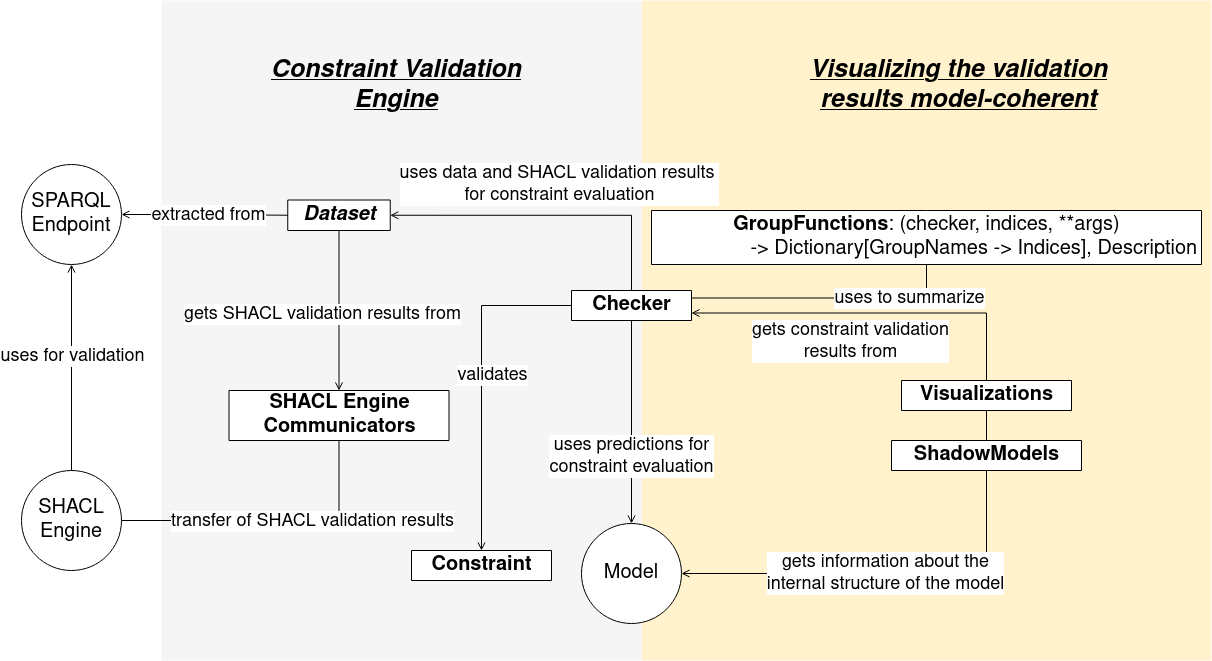
\includegraphics[scale=.35]{images/implementation/class_diagram_collapsed.png}
    \caption{Overall Structure of the Implementation}
    \label{fig:structure_of_the_implementation}
\end{figure}

Next, to give a high-level overview over the different modules, Figure \ref{fig:structure_of_the_implementation} is explained. 

On the left-hand side of Figure \ref{fig:structure_of_the_implementation}, backed in grey, the modules used to implement the constraint validation engine are depicted. These modules are capable of performing the steps described in algorithm \ref{algo:validation_engine}. 

The \textsc{Dataset} is a central module as it is responsible for storing and managing all the information collected from the endpoint and the SHACL validations, i.e., the dataset itself, the sample-to-node mapping and the SHACL validation results. Given a set of constraints, the \textsc{Dataset} initiates the process of the SHACL constraint validation.

Next is the \textsc{Checker} module, which connects the information stored in the \textsc{Dataset} with the model predictions by initiating the evaluation of the constraints. Furthermore, it stores the constraint validation results afterward.

The \textsc{SHACL Engine Communicators} and the \textsc{Constraint} module remain. The first one receives SHACL validation requests from the \textsc{Dataset}, forwards them to the SHACL engine of the user's choice, and while receiving the results transforms them to a representation independent of the chosen SHACL engine. The latter one implements the logic to evaluate a constraint given the necessary information from the \textsc{Checker} module. 

On the right-hand side of the figure, backed in yellow, the components needed to summarize and visualize the constraint validation results are shown. The \textsc{Checker} and the model partially belong to this part. The model is needed to make predictions for evaluating the constraints, but also the internal structure of the model, represented model-implementation-agnostically by the \textsc{ShadowModels} module, is used to create model-coherent visualizations of the constraint validation results.

In addition to the previously mentioned functions of the \textsc{Checker} module, it is also able to summarize the validation results in frequency distribution tables, make use of coverage and, therefore, utilizes grouping functions. Applying these concepts to constraint validation results were introduced in definitions \ref{Def:frequency_distribution_creation_function} and \ref{Def:coverage}. 
The summarized or raw validation results and the information about the internal structure of the model are then combined to create the visualization. 

The modules will be investigated further with respect to ``Performance Efficiency'' and ``Portability and Maintainability''. Both are software quality goals defined in \cite{softwarequalitygoalsiso}.



% the following selection of equally weighted software quality goals (see \cite{softwarequalitygoalsiso}):

% \paragraph{Performance Efficiency}
% The constraint validation engine and the visualization / summary process should cause as little overhead as possible. (section \ref{section_performance_efficiency})

% % \paragraph{Reliability (Explainability)}
% % An engine that validates constraints with the goal of making machine learning models more explainable should be itself explainable and transparent to the user. %TODO

% \paragraph{Portability and Maintainability (Extensibility)}
% The different modules can be extended and implementations exchanged without the need of a complete refactoring. (section \ref{section_portability_maintainability})
% % - SHACL Engine is replacable
% % - Constraints can be extended or changed semantically by inheritance
% % - ShadowModels --> Dtreeviz --> the implementation is written in a way, which allows to extend it to other implementations and other types of models.
% % - Checker
% % - GroupFunctions can be added easily and used afterwards for Frequency Distribution tables.  --> **args for further arguments

% \paragraph{Usability}
% On the one hand the implementation is simple to use, but on the other hand provides options for customization for advanced users. (section \ref{section_usability})
% % - Describe flow of using, consist of very few simple steps. --> Maybe introduce the clarify example here?
% % - Comes as a ready to start package with all it's functions documented in a sphinx documentation






% - The checker instance is choosen to be independ of the structure of the model and only depends on the needed components. Might be used in other contexts ?









% \begin{figure}
%     \centering
%     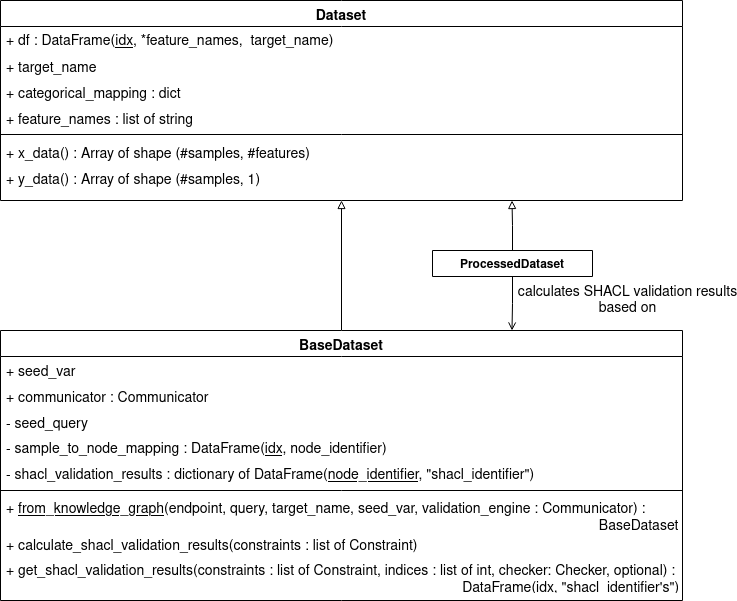
\includegraphics[scale=.35]{images/implementation/class_diagram_dataset.png}
%     \caption{Overall structure of the implementation}
%     \label{fig:package_dataset}
% \end{figure}

% \begin{figure}
%     \centering
%     \includegraphics[scale=.35]{images/implementation/class_diagram_communicators.png}
%     \caption{Overall structure of the implementation}
%     \label{fig:package_communicators}
% \end{figure}

% \begin{figure}
%     \centering
%     \includegraphics[scale=.35]{images/implementation/class_diagram_constraint.png}
%     \caption{Overall structure of the implementation}
%     \label{fig:package_constraint}
% \end{figure}


